\documentclass[CJK]{beamer}
\usepackage{CJKutf8}
\usepackage{graphicx}
\usetheme{Copenhagen}
\setbeamercovered{transparent}

\begin{document}
\begin{CJK*}{UTF8}{gbsn}

\title{Reflections on Software Research}
\subtitle{Can the circumstances that existed in Bell Labs that nurtured the UNIX project be produced again?}
\author{夏永锋}
\institute[SJTU]{上海交通大学\ 软件学院\\嵌入式实验室}
\date{\today}

\begin{frame}
	\titlepage
\end{frame}
{\tiny
\begin{frame}{About D.M.R.}
\begin{columns}
	\column{2cm}
	\begin{center}
		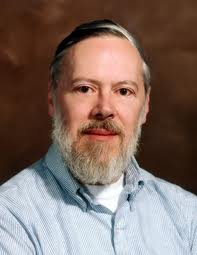
\includegraphics[width=2cm]{DMR.jpg}
	\end{center}
	\column{8cm}
	\begin{itemize}
		\item Born in Bronxville, New York
		\item Graduate from Harvard University with degrees in physics and applied mathematics.
		\item In 1967,began working at the Bell Labs Computing Sciences Research Center
		\item In 1968,received a PhD from Harvard,doctoral dissertating being "Program Structure and Computational Complexity"
	\end{itemize}

\end{columns}
	\begin{block}{Contributions}
		\begin{itemize}
			\item Creator of the C programming language
			\item A key developer of the UNIX operating system
			\item Co-author of  book "The C Programming Language" 
		\end{itemize}
	\end{block}
	\begin{block}{Awards}
		\begin{itemize}
			\item 1983, Turing Award
			\item 1990, IEEE Richard W. Hamming Medal
			\item 1997, Fellow of the Computer History Museum
			\item 1999, National Medal of Technology
			\item 2011, Japan Prize for Information and Communications
		\end{itemize}
	\end{block}
\end{frame}
}
\begin{frame}{The origin of UNIX}
	\begin{itemize}
		\item 1964: Initial planning and development for Multics started;
		\item 1969: Bell Labs pulled out of the project;
		\item 1969: Ken Thompson set out to fashion a computing environment that he liked on a little-used PDP-7 computer, then Dennis M. Ritchie joined;
		\item 1971: They acquired a PDP-11 and again implement UNIX on it;
		\item 1973: UNIX was rewritten in the C language and first described at the Operating Systems Principles conference.
		\item ...
	\end{itemize}
\end{frame}

\begin{frame}{How did UNIX come to succeed?}
	\begin{itemize}
		\item Its technical merits, especially it's a simple, coherent system that pushes a few good ideas and models to the limit.
		\item Sociological forces:
			\begin{enumerate}
				\item UNIX appeared at a time when alternatives to large, centrally administrated computation centers were becoming possible.
				\item UNIX was first available on the PDP-11, one of the most successful of the new minicomputer that appeared in the 1970s, and soon its portability brought it to many new machines as they appeared.
				\item UNIX owns much to Multics.
			\end{enumerate}
		\item UNIX enjoyed an unusually long gestation period. During much of 1969-1979, the system was effectively under the control of its designers, keep the central ideas in hand.
	\end{itemize}
\begin{block}{}
\begin{center}
Are all causes included? 
\end{center}
\end{block}
\end{frame}

{\small
\begin{frame}{The circumstances in Bell Labs}
	\begin{itemize}
		\item In Bell Labs,there is strong though wonderfully subtle pressure to think about problems somehow relevant to corporation, but researcher's interest in new idea is encouraged, and researchers does not fear edicts commanding them to be practical.
		\item The Computing Science Research Center at Bell Labs studies three broad areas: theory; numerical analysis; and systems, languages, and software, researchers can find enormous range of the puzzles that turn up.
	\end{itemize}
\begin{block}{}
The original UNIX work was not a bootleg project, it obtained management encouragement.
\end{block}
From the above, we can see that
\begin{block}{}
 Research management at Bell Labs has traditionally been sensitive to maintaining a careful balance between company interests and the industrial equivalent of academic freedom.
\end{block}
\end{frame}
}

\begin{frame}{The danger to good computer science research}
More than anything else, the greatest danger to good computer science research today may be {\bf excessive relevance.}\\
Another danger is that commercial pressures of one sort or another will divert the attention of the best thinkers from real innovation to exploitation of the current fad, from prospecting to mining a known lode.
\begin{itemize}
	\item Worldwide fascination with computers causes the best professors join start-up companies,instead of teaching.
	\item As the intensity of research in a particular area increases, so does the impulse to keep its results secret.
\end{itemize} 
\end{frame}

\begin{frame}{Alan Kay said:}
\begin{block}{}
"Atari's laboratories has lost some of the atmosphere of innovation that once attracted some of the finest talent in the industry."
\end{block}	
\begin{block}{}
"When I left last month it was clear that they would be putting their efforts in the short term."
\end{block}
\begin{block}{}
"I guess the tree of research must from time to time by refreshed with the blood of bean counters."
\end{block}
\footnote{\tiny {bean counter:数豆子的人。作为一个俗语,bean counter的意思就是一个政府官员,或者一个公司的总管老是把时间浪费在鸡毛蒜皮的小事上,尤其是为了一点点钱算计个没完。那些为政府或公司真正干些实际工作的人都很讨厌这些bean counters。}}
\end{frame}

\begin{frame}{Good research needs a long time!}
Partly because of new and immature, the arts and sciences of software abridge the chain,usual in physics and engineering between fundamental discoveries, advanced development, and application.\\
But for large systems, and for revolutionary ideas, much time is required.
\begin{block}{}
It can be said that UNIX was written in the 70s to distill the best systems ideas of the 60s, and became the commonplace of the 80s.
\end{block}
\begin{block}{}
Time, and a commitment to the long-term value of the research, are needed on the part of both the researchers and their management.
\end{block}
\end{frame}

\begin{frame}{Conclusion}
If we can keep alive  enough openness to new ideas,enough freedom of communication,enough patience to allow the novel to prosper,it will remain possible for a future Ken Thompson to find a little-used CRAY/I computer and  fashion a system as creative,and as influential,as UNIX. 
\end{frame}

\begin{frame}
	\begin{center}
	{\LARGE THANK YOU !}
	\end{center}
	\begin{block}{}
	\begin{center}
	{\small Proud to use \LaTeX\ and Beamer.}
	\end{center}
	\end{block}
\end{frame}
\end{CJK*}
\end{document}